\documentclass{standalone}
\usepackage{textcomp}
\usepackage{pgfplots}
\begin{document}
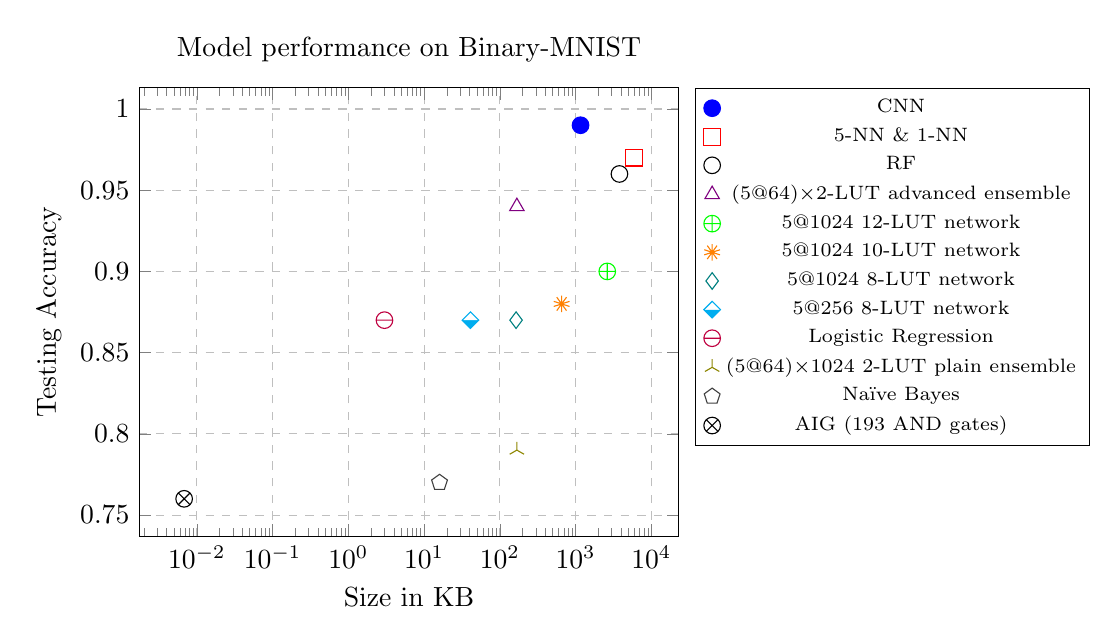
\begin{tikzpicture}
\begin{axis}[
    title={Model performance on Binary-MNIST},
    %width=0.8\textwidth,
    %height=0.5\textwidth,
    xlabel={Size in KB},
    ylabel={Testing Accuracy},
    %xmin=1, xmax=17,
    %ymin=0.44, ymax=1.1,
    %xtick={2,4,8,16,32,64,128,256,512,1024},
    %ytick={0.5,0.6,0.7,0.8,0.9,1.00},
    legend pos=outer north east,
    ymajorgrids=true,
    xmajorgrids=true,
    grid style=dashed,
    xmode=log,
    %log ticks with fixed point,
    %legend style={nodes={scale=0.5, transform shape}
    legend style={font=\scriptsize}
]

\begin{scope}[
    only marks,
    mark options={scale=1.5},
]
\addplot[
    color=blue,
    mark=*,
    ]
    coordinates {
        (1164,0.99)
    };
    \addlegendentry{CNN}

\addplot[
    color=red,
    mark=square,
    ]
    coordinates {
        (5881,0.97)
    };
    \addlegendentry{5-NN \& 1-NN}

\addplot[
    color=black,
    mark=o,
    ]
    coordinates {
        (3797,0.96)
    };
    \addlegendentry{RF}

\addplot[
    color=violet,
    mark=triangle,
    ]
    coordinates {
        (168,0.94)
    };
    \addlegendentry{(5@64)$\times$2-LUT advanced ensemble}

\addplot[
    color=green,
    mark=oplus,
    ]
    coordinates {
        (2622,0.90)
    };
    \addlegendentry{5@1024 12-LUT network}

\addplot[
    color=orange,
    mark=10-pointed star,
    ]
    coordinates {
        (655,0.88)
    };
    \addlegendentry{5@1024 10-LUT network}

\addplot[
    color=teal,
    mark=diamond,
    ]
    coordinates {
        (164,0.87)
    };
    \addlegendentry{5@1024 8-LUT network}

\addplot[
    color=cyan,
    mark=halfsquare*,
    ]
    coordinates {
        (41,0.87)
    };
    \addlegendentry{5@256 8-LUT network}

\addplot[
    color=purple,
    mark=halfcircle,
    ]
    coordinates {
        (3,0.87)
    };
    \addlegendentry{Logistic Regression}

\addplot[
    color=olive,
    mark=Mercedes star,
    ]
    coordinates {
        (168,0.79)
    };
    \addlegendentry{(5@64)$\times$1024 2-LUT plain ensemble}

\addplot[
    color=darkgray,
    mark=pentagon,
    ]
    coordinates {
        (16,0.77)
    };
    \addlegendentry{Naïve Bayes}

\addplot[
    color=black,
    mark=otimes,
    ]
    coordinates {
        (0.0068,0.76)
    };
    \addlegendentry{AIG (193 AND gates)}

%\addplot[
    %color=red,
    %mark=square,
    %]
    %coordinates {
        %(0.0004,0.50)
    %};
    %\addlegendentry{Random Guess}
\end{scope}

\end{axis}
\end{tikzpicture}
\end{document}
